\documentclass[11pt]{article}

\usepackage[a4paper]{geometry}
\geometry{left=2.5cm,right=2.5cm,top=2.5cm,bottom=2.5cm}

\usepackage{comment}
\usepackage{booktabs}
\usepackage{diagbox}
\usepackage{amsmath,amsfonts,graphicx,amssymb,bm,amsthm}
\usepackage{algorithm,algorithmicx}
\usepackage[noend]{algpseudocode}
\usepackage{fancyhdr}
\usepackage{subfigure} 
\usepackage{tikz}
\usepackage{graphicx}
\usetikzlibrary{arrows,automata}
\usepackage{hyperref}
\usepackage[font=scriptsize]{caption}

\setlength{\headheight}{14pt}
\setlength{\parindent}{0 in}

\title{Proposal}
\usetikzlibrary{positioning}

\begin{document}
%\pagestyle{fancy}
%\lhead{Brown University}
%\chead{}
%\rhead{DATA 1030, 2021 Fall}

\begin{center}
	{\LARGE \bf   COVID-19 Total Cases Prediction on Country-based Multivariable Time Series}\\
	\vspace{0.3cm}{Nange Li}
\end{center}

\section{Introduction}
% background
\subsection{Background}
Since the beginning of the year 2020, the spreading coronavirus disease 2019 (COVID-19) has aroused global concern on public health and people's lives. In order to closely monitor the nation-wise situation and reduce prevalence, many governments are trying to collect everyday data on new positive cases, death rates, and encouraging citizens to complete vaccinations. Under the travel ban of several major countries and the fast increasing vaccination rate, the world witnessed an outcome in combating the spread. However, today our world is still under the threaten of the COVID-19 pandemic. Predicting the future trend would be necessary as this is a base for short or long-term policies establishment.

\subsection{Dataset}
This project will employ the dataset maintained by {\em Our World in Data [1]} (OWID). While the data is fundamentally collected case-by-case, individual information regarding specific patients is not included in OWID's dataset. For each country or region, the daily-updated dataset has 65 columns, 122636 records (up to Oct 6th, 2021) covering every day updated COVID observations, demography statistics, as well as economic data of 233 countries.  Hence, this project will focus on the statistical information mined from the dataset, apply time series analysis and regression models to predict the future trend of total confirmed COVID-19 cases. \\

% previous works
Researchers on the OWID dataset have implemented both mathematical models and machine learning models. In 2020, Valvo et al. [2] developed a bimodal lognormal distribution model for a country's time distribution of deaths. In the same year, Shreshth et al. [3] also applied the model to country-based data.  They proposed a novel method using machine learning and cloud computing to improve the performance of pure mathematical models and predict the impact of the COVID-19 pandemic. 

\begin{figure}[htb]
	\setlength{\abovecaptionskip}{-0.5cm}
	\centering
	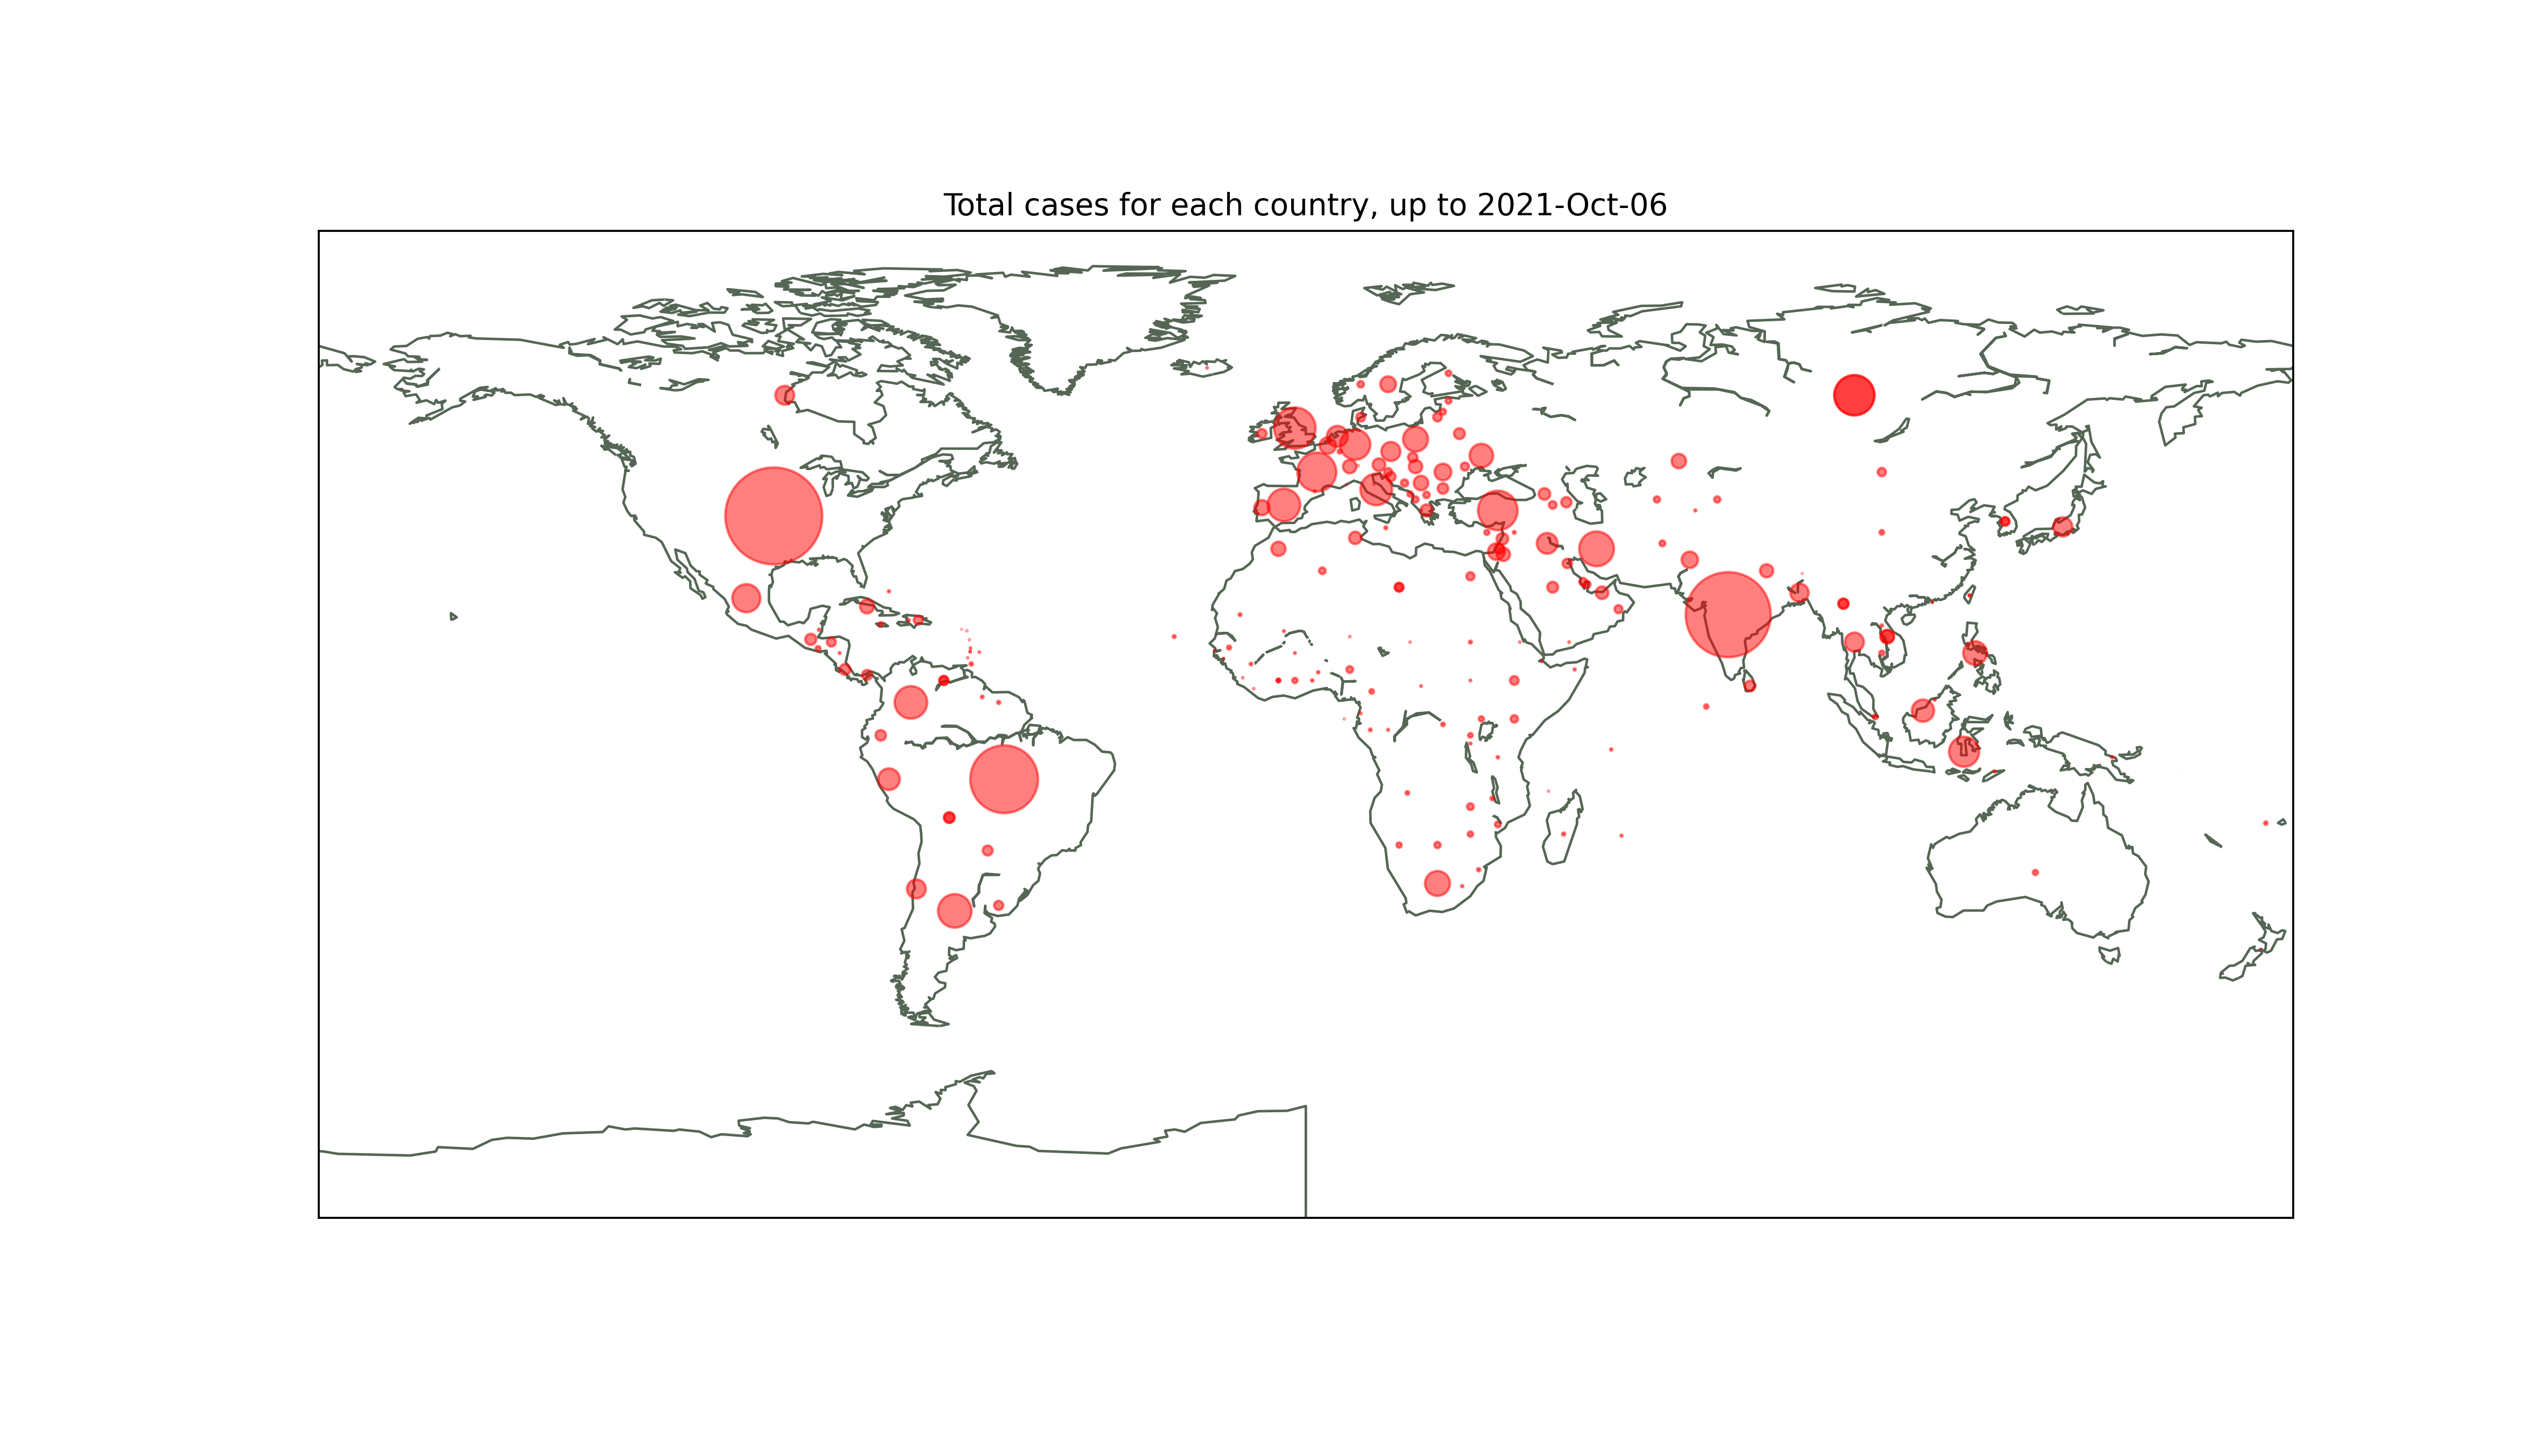
\includegraphics[width=0.8\linewidth]{../figures/total-cases-map.png} % Figure image
	\caption{This figure displays the total confirmed COVID-19 cases (up to Oct 6th, 2021) of each country. Each red dot represents a country's total cases, placed at the averaged latitude and longitude. The size of the dot is the number of the total cases scaled by a factor of 30,000. From this figure, countries with the most cases are the US, India, and Brazil.} % Figure caption
\end{figure}

\section{Exploratory Data Analysis}
Figure 1, 2, and 3 are included in this report visualizing the information extracted from a thorough EDA process. 

\begin{figure}[htb]
	\setlength{\abovecaptionskip}{0.cm}
	\centering
	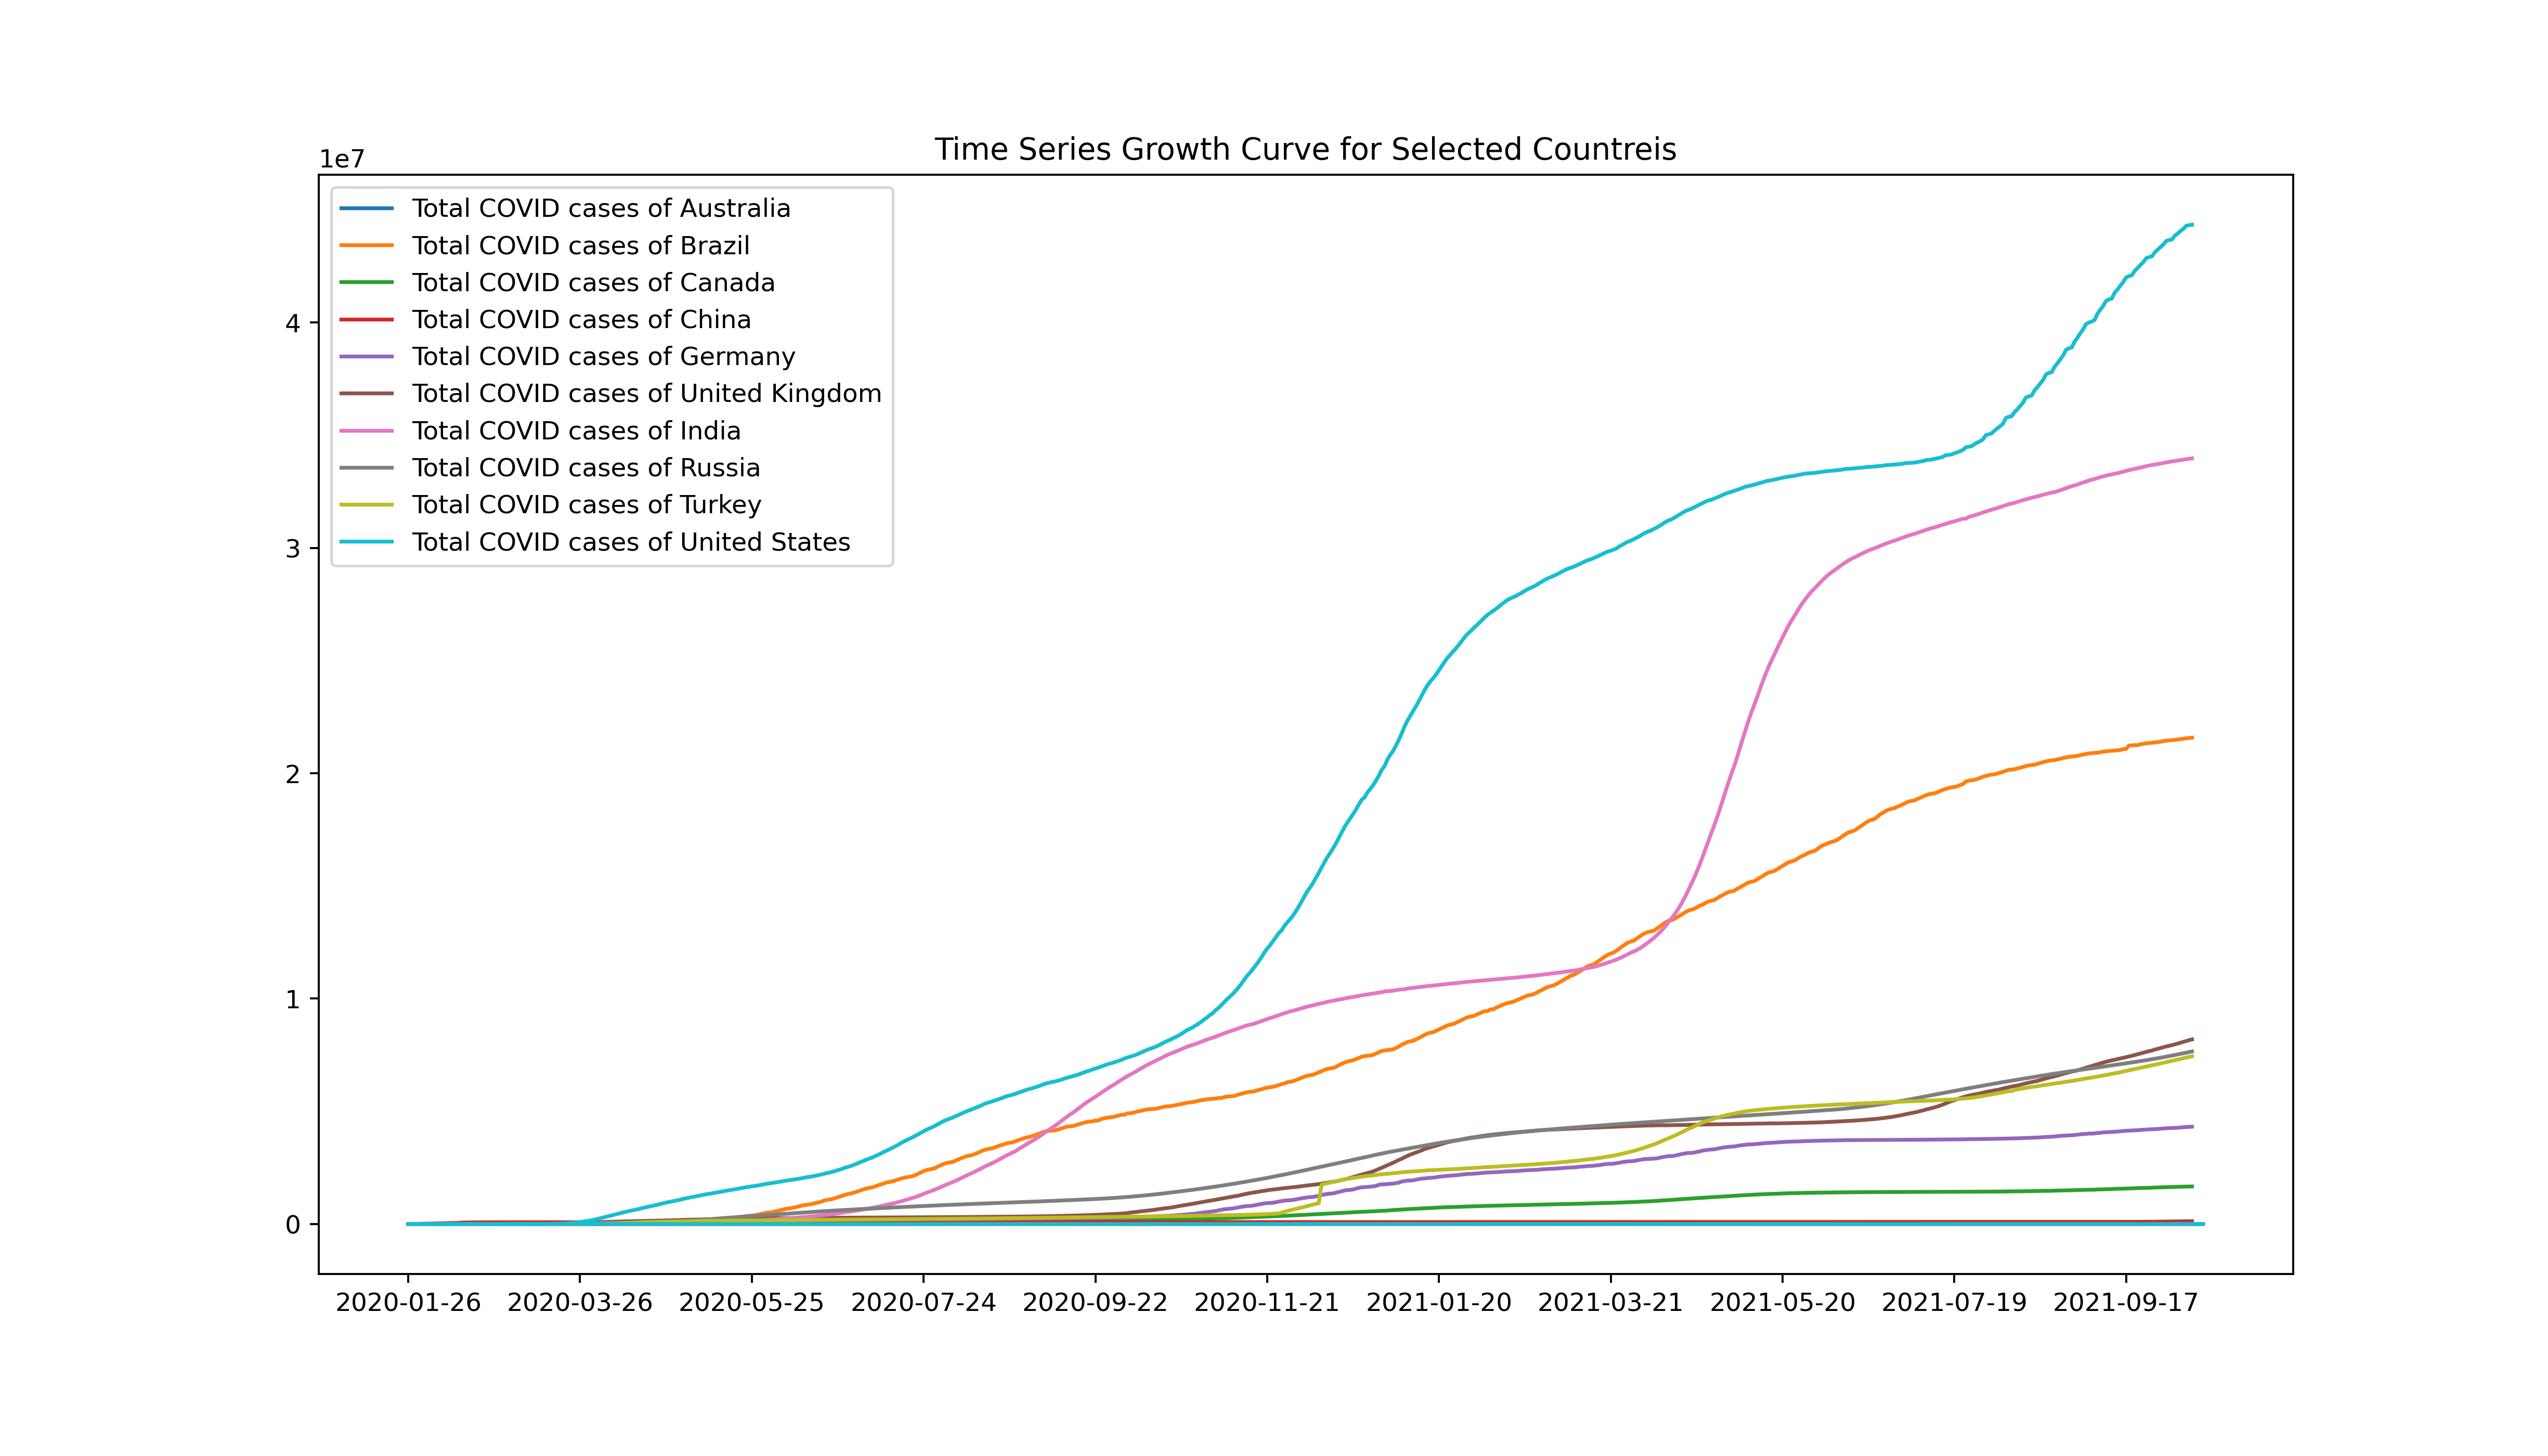
\includegraphics[width=0.8\linewidth]{../figures/total-cases-time-series.png} % Figure image
	\caption{Here ten countries are selected from 233, and this figure displays the growth curve of total cases from Jan 2020 to Oct 2021. While the curve of total cases of China, Australia, and even Canada, are kept relatively low and stable, the curve, unfortunately, goes up rapidly in the US, India, and Brazil, which also accounts for their most cases in Figure 1.} % Figure caption
\end{figure}


\begin{figure}[htb]
	\centering
	\subfigure[total cases vs. new cases]{
		\label{total cases vs. new cases} 
		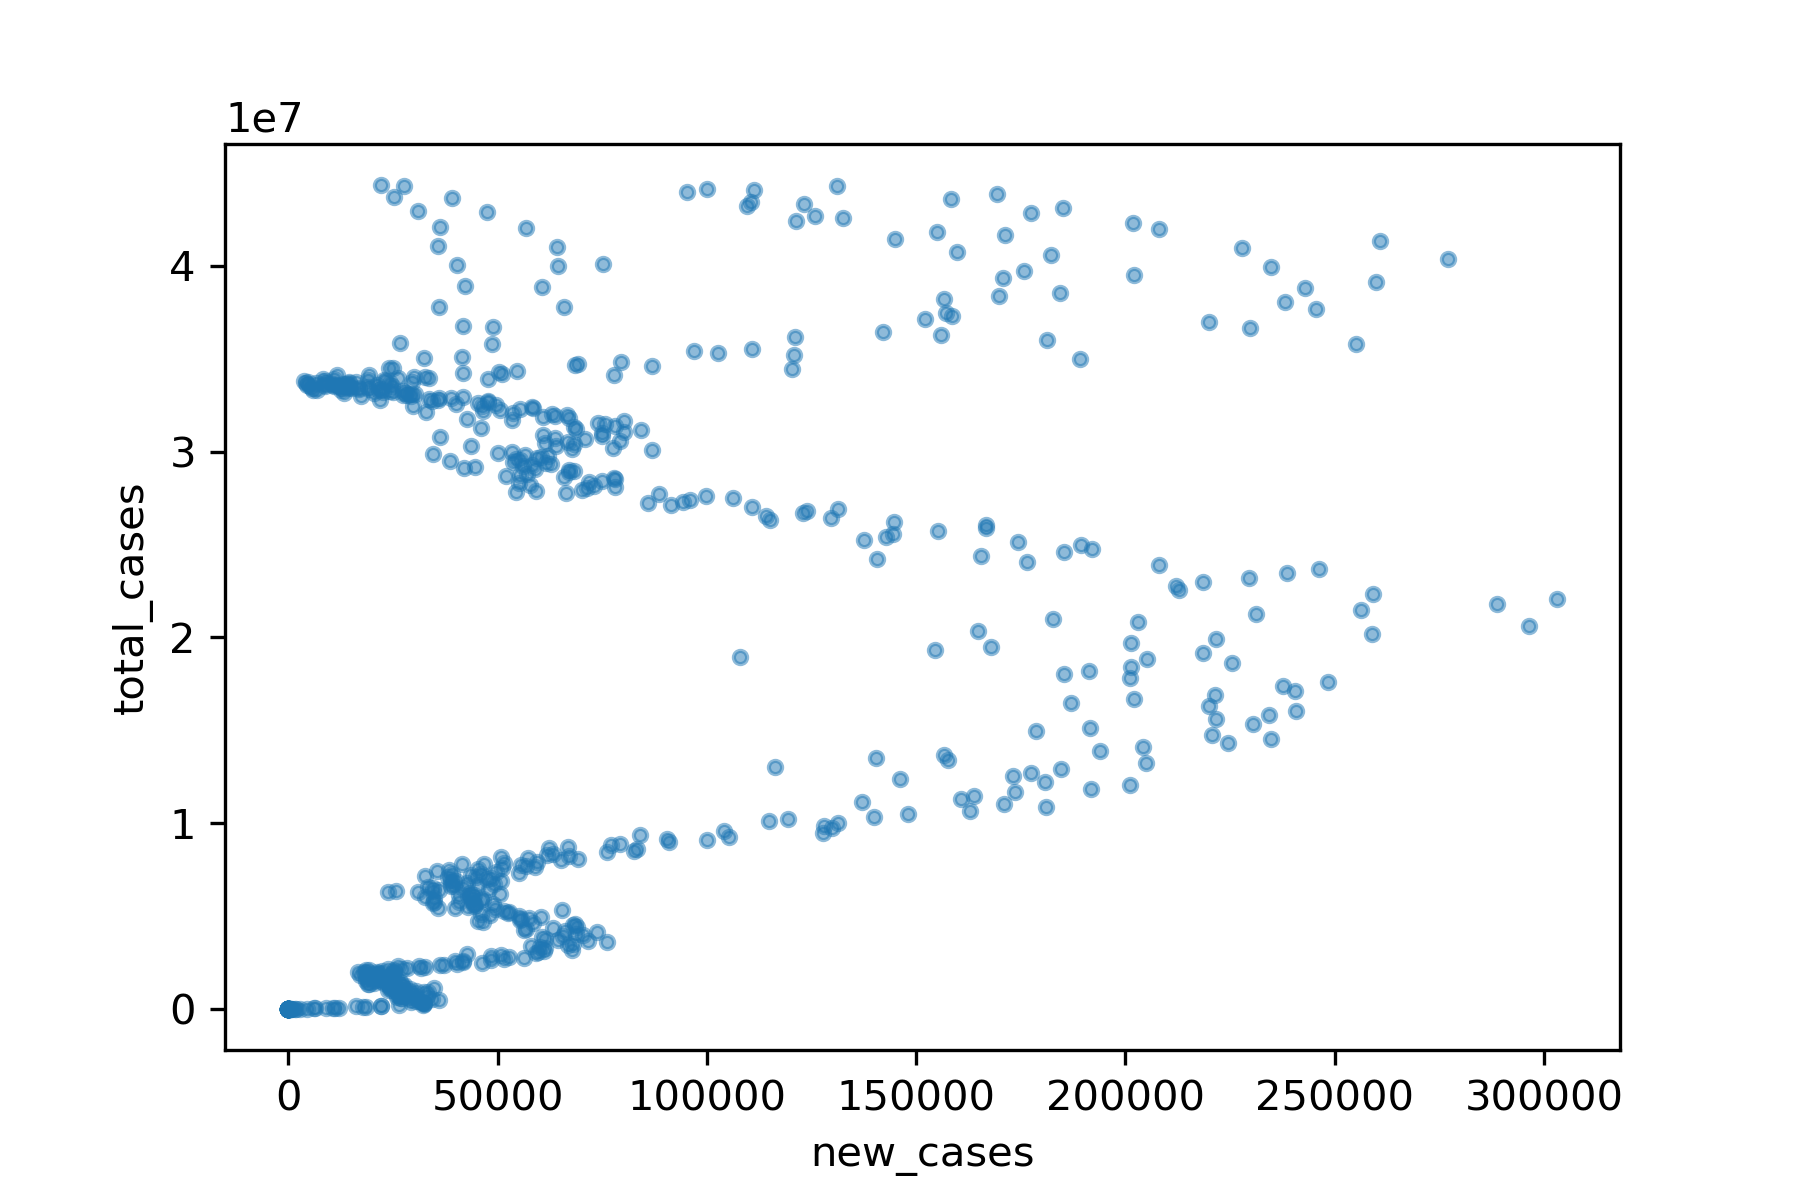
\includegraphics[width=0.45\textwidth]{../figures/total_cases-new_cases-scatter.png}}
	\subfigure[total cases vs. cumulated new cases]{	
		\label{total cases vs. cumulated new cases} %% label for secondsubfigure
		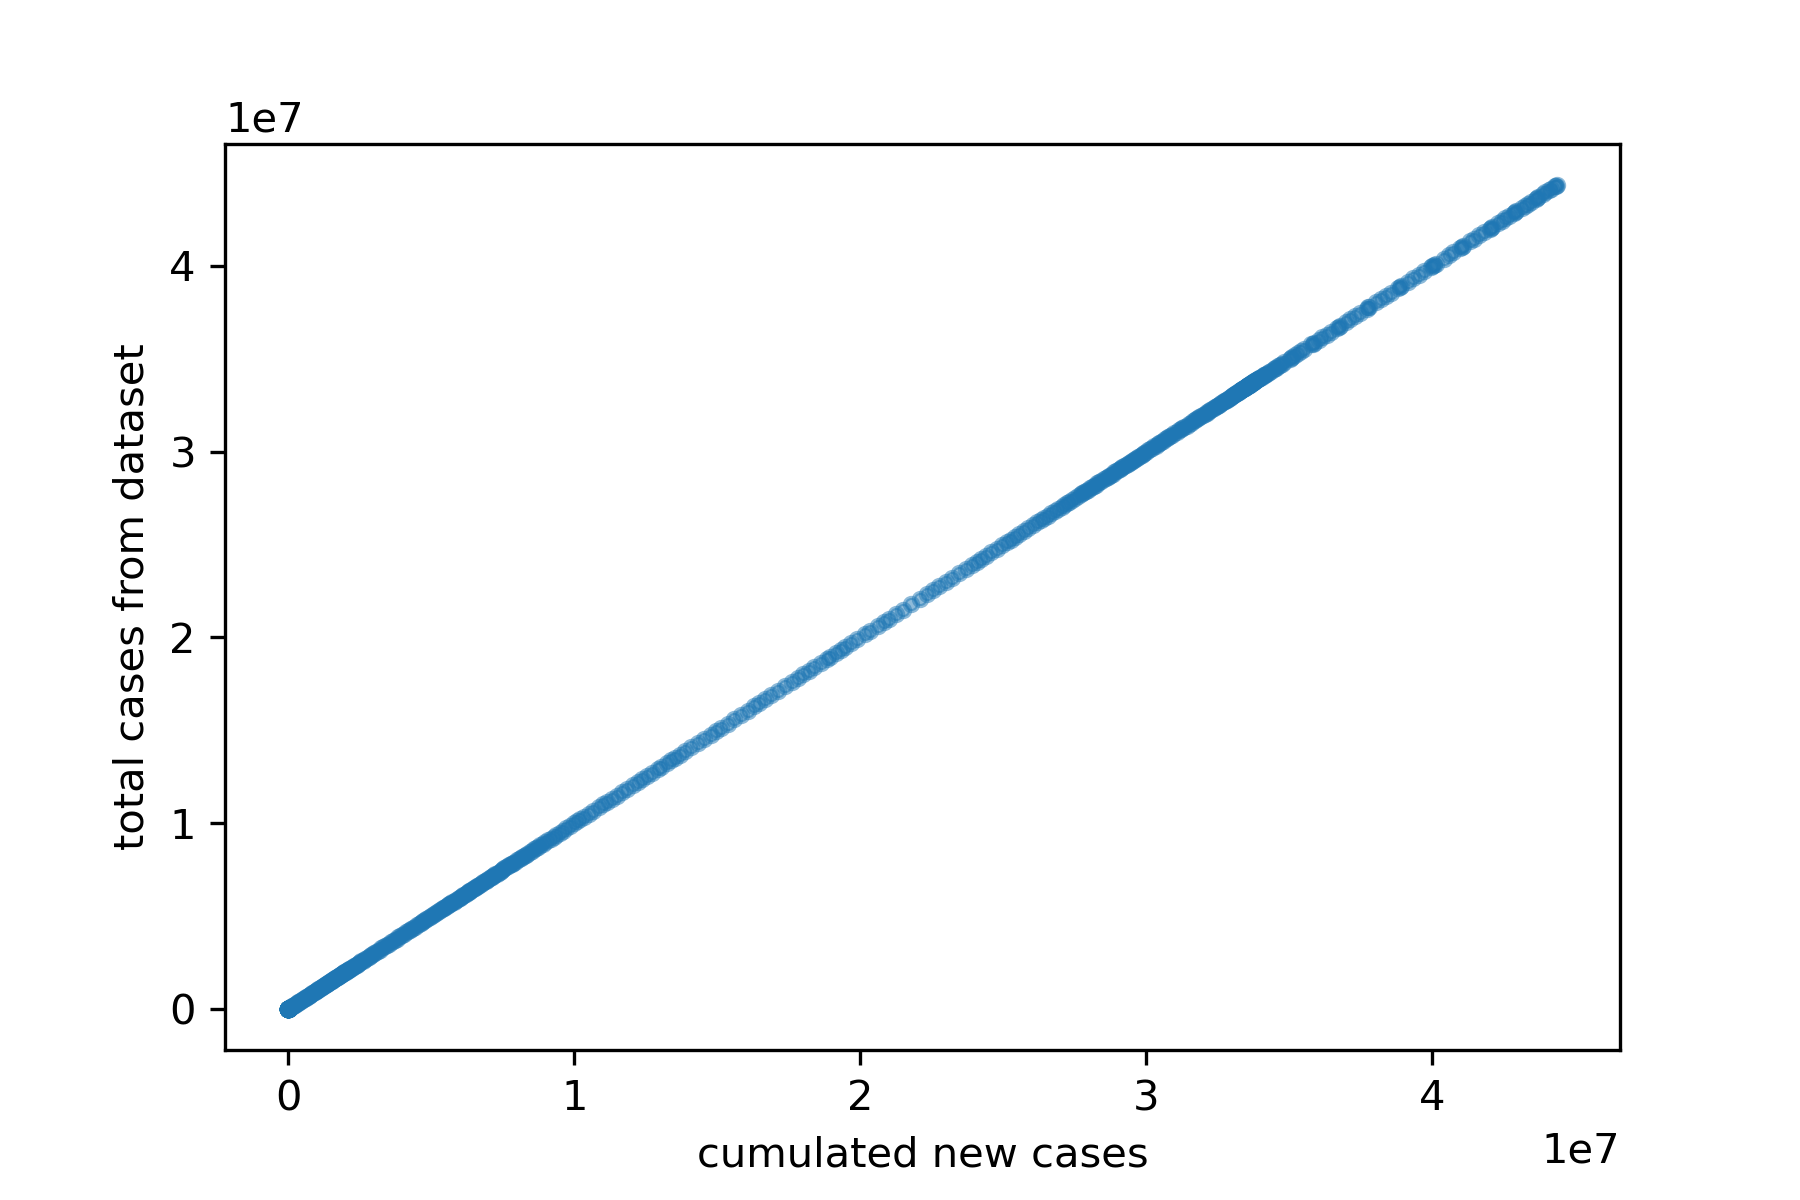
\includegraphics[width=0.45\textwidth]{../figures/total_cases-manual-scatter.png}}
	\caption{While there are 65 columns, including our target variable of total cases and 64 feature variables, not all the features can be applied for future prediction. This figure shows a scatter between total cases and new cases data, with two variables convertible into each other - new cases series is the first-order difference of total cases series, and by cumulating the former we can easily recover the latter series. Though from (a) it is not apparent to get this conclusion that the two series share the same information, after manually summing the new cases, (b) displays a straight line, where the Pearson correlation coefficient between manual cumulated new cases and total cases is precisely 1.0.)}
\end{figure}

\section{Modeling}
\subsection{Data Preprocessing}
In feature selection, the first three columns are indexing countries, so they are set as keys when grouping data. The date column is then set as an index on the grouped set of one country since the series has already been timely ordered. Also, columns directly connected to the target variable (those concerning new cases data) are eliminated from the selected features. After these steps, there are 54  features elected for the following process, among which 17 features have more than 80\% missing values.\\

As the dataset combines group and time series structure, the splitting is performed on time series grouped by country names. For time series, we should never use future information on validation or test, so the training set can only have records previous to records in the test set. And K-Fpld cross-validation is also a bit special for time series. While 10\%  latest records are divided into test sets, and in a loop for K-Fold, 90\% rest data in which one fraction following the training time period is separated into validation set. The test and validation set keep the same size all the time, and training set is growing in each iteration. \\

StandardScaler is applied to the selected features inside the loop of K-Fold. While features are not strictly continuous, like the test cases and deaths only contain integers, it still makes sense to approximate those features with continuous variables instead of ordinal data, transferring the exact number to a kind of ratio. 

\begin{thebibliography}{99}
	\bibitem{1}Ritchie, H., Mathieu, E., et al. 2020. "Coronavirus Pandemic (COVID-19)". Published online at {\em OurWorldInData.org}. Retrieved from: \url{https://ourworldindata.org/coronavirus}
	\bibitem{2}Valvo, \& Paolo S. 2020. A Bimodal Lognormal Distribution Model for the Prediction of COVID-19 Deaths" {\em Applied Sciences }10, no. 23: 8500. \url{https://doi.org/10.3390/app10238500}
	\bibitem{3} Tuli, S., Tuli, R., Gil, S S., 2020. "Predicting the growth and trend of COVID-19 pandemic using machine learning and cloud computing". {\em Internet of Things},
Volume 11,
2020,
100222,
ISSN 2542-6605,
	\url{https://doi.org/10.1016/j.iot.2020.100222}.
\end{thebibliography}
\subsubsection*{GitHub repository } 
\url{https://github.com/7ericany/1030Project/tree/master}
\end{document}

